\documentclass[12pt,a4paper,oneside]{report}
\usepackage[utf8x]{inputenc}
\usepackage[brazilian]{babel}
\usepackage{url} % para formatar URLs no documento
\usepackage{amsmath} %include de estilo de equações matmáticas
\usepackage{graphicx} %biblioteca de imagens
\usepackage{indentfirst}
\usepackage{sidecap}
\usepackage{setspace}
\doublespacing

%ctan.org
%wikibooks - tem um para latex
%Alt + 1 = compila e executa
\usepackage{setspace}
\doublespacing
\begin{document}

%opening
\title{Implementação e avaliação de cenário de convergência telefonia-rede integrando serviços de VoIP e video-chamada com o uso de WebRTC}
\author{Rafael Ossamu Togo \\ \\ Orientador: Prof. Arliones Hoeller} % o comando \\ pula linha 
\date{Julho 2014}

\maketitle %cria o artigo e o autor deste

\tableofcontents 

\begin{abstract}
O WebRTC \textit{Web Real Time Communication} permite a transmissão de áudio vídeo e compartilhamento de dados entre usuários que utilizem um simples navegador, de maneira nativa. Como um conjunto de normas, WebRTC proporciona a qualquer navegador a capacidade de compartilhar dados e realizar teleconferência peer to peer, sem a necessidade de instalar plugins ou software de terceiros. WebRTC não vem adicionar novos serviços à
rede, mas sim tornar a sua utilização mais fácil

Este documento aborda as tecnologias necessárias para o desenvolvimento de uma aplicação, que tem como objetivo realizar a integração de serviços de VoIP, com o uso do WebRTC. Apontar as vantagens e desvantagens frente as atuais tecnologias,  e avalia o desempenho do sistema utilizando esta tecnologia.  

\end{abstract}


\chapter{Introdução} % artigo é dividido por sessões
\label{c_introducao} % serve para referência cruzada
Entendemos que a Internet revolucionou a forma como as pessoas vivem e se relacionam, porém a maneira em que hoje a enxergamos a Web (World Wide Web), demandou um certo tempo de amadurecimento, no que diz respeito a organização, estruturação e padronização.
 
Em 12 de março de 1989, Tim Berners-Lee divulgou no interior da Organização Europeia para a Pesquisa Nuclear (CERN) um projeto baseado no conceito de hipertexto para facilitar o compartilhamento e a atualização de informações apenas entre os pesquisadores da própria organização. Deu-se então o surgimento do que viria a se tornar a World Wide Web (WWW). 

Com a Web em processo de evolução, em 1994 surge a W3C World Wide Web Consortium  que torna-se o órgão oficial para a gestão da Internet e padrões da web como HTML (HyperText Markup Language) e CSS (Cascading Style Sheets), em todo o mundo, tornando a página web melhor estruturada e organizada.

Com o passar do tempo, diversas diretrizes, recomendações e normas da W3C foram surgindo, tornando uma página Web um ambiente maduro para desenvolvimento, permitindo a diversos desenvolvedores criarem suas próprias aplicações. 

Diretamente no ano de 2012, com a ajuda da W3C e da The Internet Engineering Task Force (IETF)  foi possível criar uma tecnologia que permite comunicação em áudio e vídeo diretamente entre web browsers, resultando no chamado \textit{Web Real Time Communication}(WebRTC). Esta tecnologia permite que haja comunicação em tempo real, com voz, vídeos e dados, utilizando apenas navegadores web, não havendo necessidade de instalação de plugins ou softwares, como é o caso do Skype, eBuddy e Numbuzz, nem da intermediação de servidores para troca de dados.
	
Em uma época onde temos cada vez mais serviços rodando na nuvem, essa tecnologia tem tudo para se tornar a base de soluções de comunicação em tempo real, fazendo com que muitas empresas hoje consolidadas busquem pelo mesmo tipo de solução para não perderem espaço no mercado.

\section{Motivação}
\label{s_motivacao} %serve para referência cruzada
O fato do WebRTC permitir estabelecer comunicação por som e imagem (video-conferência), de browser para browser, sem necessidade de nenhum outro plugin ou software, já o torna atraente para as futuras aplicações. Ou seja, a tendência para as próximas aplicações que utilizarem esta tecnologia, é tornar a comunicações entre os usuário, cada vez mais prática e eficaz. É por esse tipo de solução que os usuários tem buscado fortemente. 

Este trabalho também busca dar continuidade a um TCC desenvolvido anteriormente no IFSC-SJ por Felipe Borges intitulado \textit{Webrtc: Estudo e análise do projeto} \cite{Borges:2013}.


\section{Objetivos}
\label{s_objetivos} %serve para referência cruzada
O objetivo deste trabalho é implementar e avaliar um cenário típico de convergência telefonia-rede integrando serviços de VoIP e video-chamadas, utilizados a partir de navegadores Web  com suporte ao WebRTC. Neste cenário será desenvolvido uma aplicação onde um usuário encontrará outros que estarão disponíveis (online) em sua lista de contatos, para então iniciar uma chamada. 

\subsection{Objetivos Específicos}
\label{ss_objEspecicos}

\begin{itemize} %Latex < List Environment
 \item Implementar test-bed de infraestrutura de controle de VoIP e Videoconferencia com Asterisk.
 \item Desenvolver/buscar um mecanismo de divulgação de usuários disponiveis.
 \item Realizar testes utilizando a rede do Campos IFSC/SJ.
 \item Criar uma interface amigável e intuitiva aos usuários, para lidar com a aplicação desenvolvida.
 \item Avaliar o desempenho do sistema.
\end{itemize}


\section{Metodologia}
\label{s_metodologia} %serve para referência cruzada

Através das linguagens HTML, CSS e Javascript, é necessário criar uma interface amigável e intuitiva aos usuários, para que estes possam interagir entre sí, sem grandes dificuldades. Essa interação ocorrerá de três maneiras: chamadas de áudio, video e texto.

Após a criação da aplicação, haverá a integração do sistema com o Asterisk, pois toda a sinalização será através de SIP. É preciso criar um método que irá coletar todos os usuários que estão registrados, e mostrar quem está \textit{online}.

Será necessário o uso de máquinas virtuais para simulação dos usuário, do servidor Asterisk e outra para a própria aplicação. Serão testados os protocolos ICE, STUN, TURN, protocolos que auxiliarão vários clientes trocarem informação mídia através de NAT.

Com o cenário já montado, serão realizados testes para avaliar o desempenho e qualidade de serviço implementado.


\chapter{Fundamentação Teórica} % artigo é dividido por sessões
\label{c_fundamentacaoTeorica} % serve para referência cruzada

Este capítulo apresenta a fundamentação teórica do trabalho, inclui o estudo e descrição das tecnologias que serão importantes para o desenvolvimento do projeto. 

\section{WebRTC}
\label{c_webRtc} 


O WebRTC é um projeto de código aberto que permite aplicações de comunicação em tempo real, com voz, vídeos e dados, utilizando apenas navegadores web, não havendo necessidade de instalação de plugins ou softwares.

Oferece aos desenvolvedores meios para desenvolver aplicações em tempo real de maneira prática e auxilia na construção de uma plataforma RTC \textit{Real-Time Communications} que funciona em diversos navegadores através de múltiplas plataformas.

O papel fundamental do WebRTC é disponibilizar funções e recursos para que o desenvolvedor web possa implementar uma aplicação que funcione como um telefone ou uma unidade de vídeoconferência, pois o WebRTC nada mais é que um \textit{média engine}\footnote{Responsável por realizar o tratamento da mídia} que faz interações com API's Javascript e com o próprio sistema operacional do usuário, para ter acesso aos recursos de câmera e microfone.

Outras funções que são de responsabilidade de um navegador com suporte a WebRTC, é a codificação/decodificação das mídias que serão utilizadas, bem como funções de processamento de mídia como cancelamento de eco entre outras.

\section{Arquitetura do WebRTC}
\label{s_webRtc}
A arquitetura do WebRTC é constituida por duas camadas. A primeira é denominada Web API, onde é disponibilizada funções para que os desenvolvedores Web possam desenvolver suas aplicações. A segunda é o WebRTC C++ API, a qual é utilizada para o desenvolvimento de browsers. A Figura 2.1 demonstra a arquitetura do WebRTC, com suas camadas e blocos.

\begin{figure}[!htdb]
 \centering
  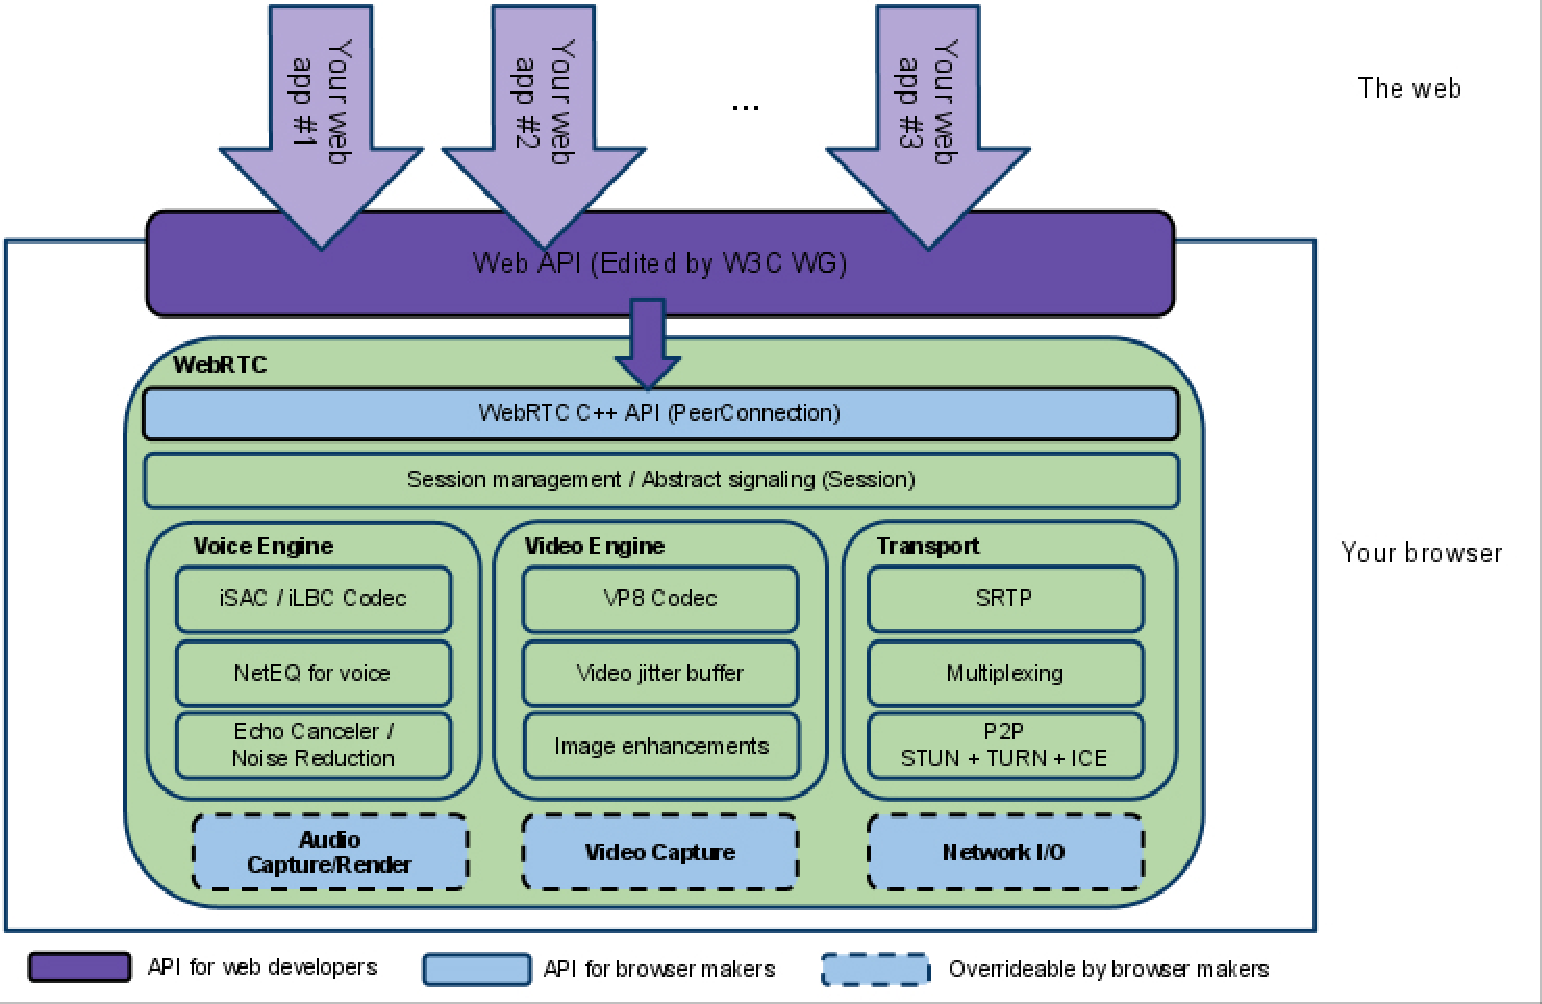
\includegraphics[width = 1.2\linewidth]{images/webrtcArchitecture}
  \caption{Arquitetura do WebRTC} %titulo da figura
  \label{f_webrtcArquitetura}
\end{figure}

\subsection{Web API}
\label{ss_webApi}
Utilizando o Javascript, esta API permite o desenvolvimento de aplicações de comunicação em tempo real em web browsers. Podemos dividir em três partes: \textit{MediaStream}, \textit{PeerConnection} e \textit{DataChannels}.

\subsubsection{MediaStream}
\label{sss_mediaStream}
Utilizando a função \textit{getUserMedia()}, esta API é responsável por solicitar acesso ao microfone e câmera do usuário para a geração de uma \textit{stream} de dados. Esta \textit{stream} será enviada utilizando o protocolo de transporte \textit{Secure Real-time Transport Protocol} (SRTP), no qual é umas das exigências no uso do WebRTC. Exemplo de funcionamento na figura 2.2.

\begin{figure}[!htdb]
 \centering
  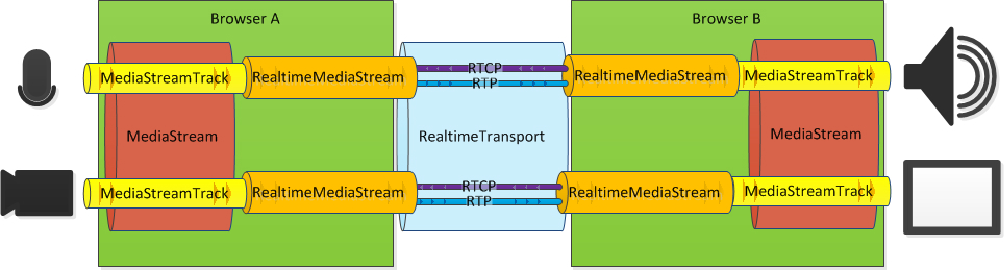
\includegraphics[width = 1.1\linewidth]{images/mediaStream}
  \caption{Captura e envio da stream para outro usuário} %titulo da figura
  \label{f_mediaStream}
\end{figure}

O código abaixo (Figura 2.3), mostra de maneira simples, como é feita a captura da mídia de um usuário. Neste exemplo, é solicitado apenas áudio para ser enviado para outro destino. 

\begin{figure}[!htdb]
 \centering
  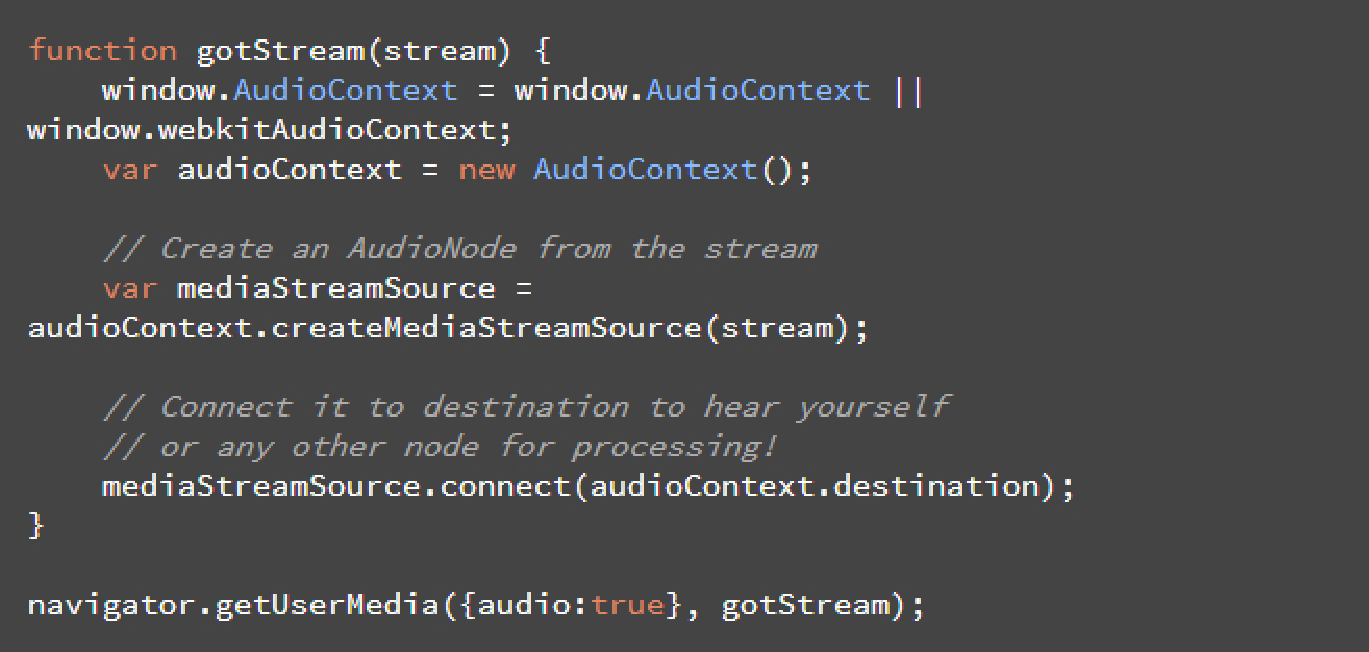
\includegraphics[width = 1\linewidth]{images/mediaStreamCode}
  \caption{Função de captura de mídia} %titulo da figura
  \label{f_mediaStreamCode}
\end{figure}

Na última linha, o método \textit {navigator.getUserMedia()}, solicita o acesso ao microfone do usuário. Logo em seguida ele chama a função \textit {gotStream()} para gerar uma stream de dados, que pode ser enviado a algum destino específico.

\subsubsection{PeerConnection}
\label{sss_peerConnection}
Esta API é quem estabelece uma conexão entre dois browsers, faz o controle do codec que será utilizado, criptografia e gerenciamento de banda. Ou seja, protege os desenvolvedores web de diversas complexidades que existem, ao se fazer uma conexão \textit{browser-to-browser} Para estabelecer esta conexão, é necessário um canal para a sinalização. Este é implementando num servidor, utilizando WebSockets ou XML-HttpRequest.

\subsubsection{DataChannel}
\label{sss_dataChannel}
Para a transferência de dados diretamente de um ponto a outro, utilizamos a API DataChannel. Entende-se como dados: 
\begin{itemize}
  \item Transferência de arquivos
  \item Mensagens instantâneas
  \item Compartilhamento de tela
\end{itemize}
Tem como expectativa o desempenho e baixa latência de conexão entre dois clientes. Pode-se utilizar tanto TCP \textit{Transmission Control Protocol}, causando velocidades mais lentas porém garantido, ou UDP \textit {User Datagram Protocol}, para velocidades mais rápidas com possível perda de pacotes.

\subsection{WebRTC C++ API}
\label{ss_webrtcAPI}
Esta API é voltada exclusivamente para o desenvolvimento de browsers, na implementação do WebRTC. A WebAPI é open source e está disponível para qualquer desenvolvedor que queira realizar a integração de seus produtos com os padrões WebRTC. Este trabalho não trabalhará em cima desta API.

\subsection{Voice Engine}
\label{ss_voiceEngine}
Como foi visto na imagem 2.1, o Voice Engine é um dos mecanismos que formam o WebRTC. É responsável desde a captura do áudio da placa de som, tratamento e envio para a interface de rede. Cancelamento de eco, redução de ruído e uso de codecs específicos.

\subsection{Video Engine}
\label{ss_videoEngine}
Responsável pela captura da imagem da \textit{WebCam}, para que esta seja enviada pela \textit{web}. Também é responsável pelo seu tratamento, reduzindo a quantidade de ruído da imagem.
Até hoje não foi definido qual codec de vídeo que será utilizado, pois ainda existe uma grande disputa comercial em torno deste assunto. A disputa hoje está entre o VP8 e o H.264. 

Em questão de qualidade e consumo de bateria, o H.264 é considerado superior, pois os processadores de vídeo atuais possuem hardwares dedicados para codifica-los, ao contrário do VP8, onde a codificação é feita através de software, consumindo uma quantidade considerável da bateria. Em favor do VP8 e uma das premissas do WebRTC desde o seu princípio, é que este está livre de \textit{royalties}\cite{Borges:2013}.

\subsection{Transport}
\label{ss_videoEngine}
Em relação ao transporte da mídia, o WebRTC faz uso do SRTP, que tem como função criptografar a mídia para que esta não seja criptografada por terceiros.

Para clientes que estão por trás de NAT, há necessidade da utilização dos protocolos ICE, STUN e TURN para auxiliar no envio da mídia. 

\subsubsection{\textit{Interactive Connectivity Establishment(ICE)}}

O ICE é um protocolo para travessia de NAT para \textit{streams} de mídia, estabelecidas sob o modelo Oferta e Resposta. Surgiu com o intuito de servir com uma solução geral para diversas topologias de rede, resolvendo o problema de desenvolvedores e administradores de rede que precisam fazer suposições e estudo a respeito das topologias onde seus sistemas serão implantados\cite{Varanda:2008}.

O modelo de Oferta e Reposta apresenta algumas dificuldades em operar através de NAT, pois para estabelecer um fluxo de mídia entre dois usuários é trocado entre eles mensagens de endereços IP e portas, que não são tratados corretamente pelos dispositivos de NAT.

Para viabilizar o estabelecimento de conexões multimídia entre dois usuários, o protocolo ICE pode tirar proveito ou compor as funcionalidades de outros protocolos, neste caso o STUN e TURN. 

Em relação ao WebRTC, este protocolo permite a troca de mídia entre dois clientes que estejam por trás de NAT.

\subsubsection{\textit{Session Traversal Utilities for NAT (STUN)}}

O STUN, juntamente com o protocolo ICE, apresentam uma solução integral para a questão de travessia de NAT. Ele permite a um agente descobrir qual porta e endereço IP externo está mapeado para seu endereço IP e porta interno, ou seja, permite que a ligação NAT permaneça ativa\cite{Varanda:2008}. 

Na tecnologia WebRTC, o STUN é utilizado para estebelecer a sessão entre dois clientes, onde o \textit{web browser} funciona como um cliente STUN e o servidor web como servidor STUN, e são enviados pacotes de testes para mapear as portas e endereços IP por trás de NAT. Exemplo na figura 2.4.

\begin{figure}[!htdb]
 \centering
  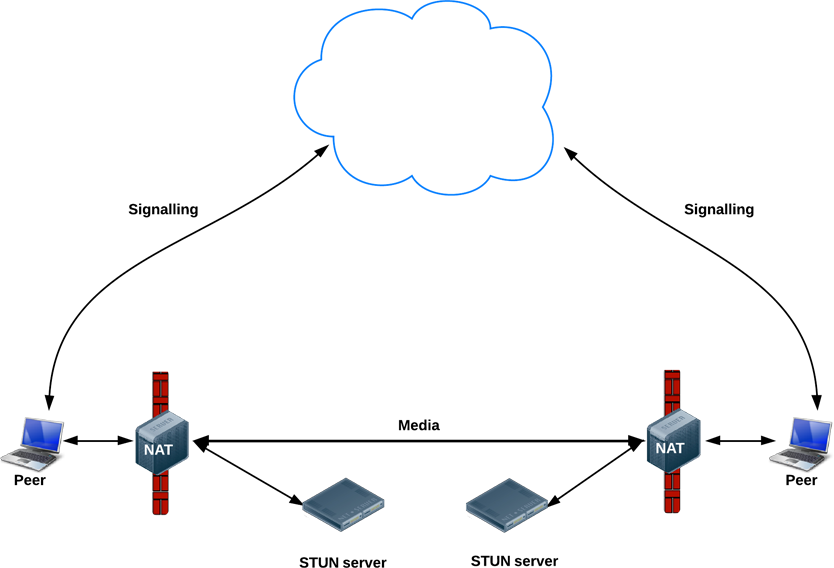
\includegraphics[width = 1\linewidth]{images/stun}
  \caption{Cenário utilizando o protocolo STUN} %titulo da figura
  \label{f_mediaStream}
\end{figure}

\subsubsection{\textit{Traversal Using Relays around NAT (TURN)}}

Quando não há possibilidade de estabelecer um canal direto entre dois agentes posicionados atrás de um NAT, é necessário recorrer a um host intermediário, que irá agir como um \textit{relay}. Este normalmente se encontra na rede pública e tem a função de retransmitir os pacotes entre os agentes\cite{Varanda:2008}. Exemplo de utilização na figura 2.5.


\begin{figure}[!htdb]
 \centering
  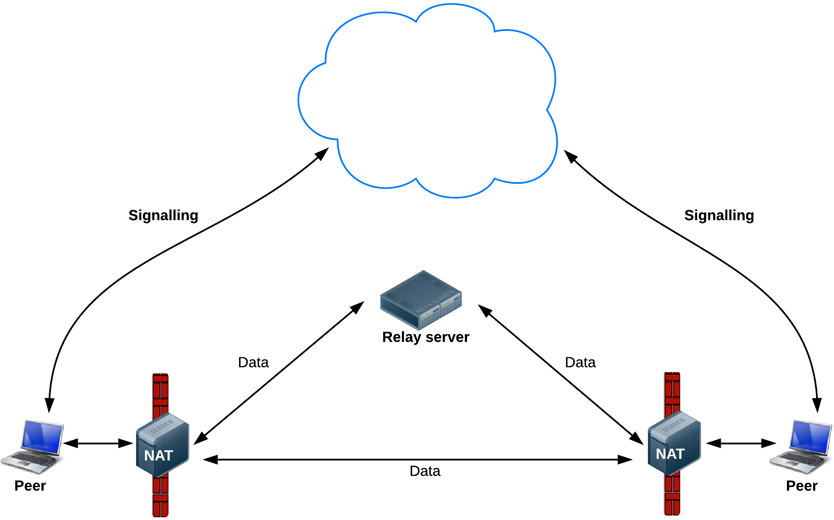
\includegraphics[width = 1\linewidth]{images/turn}
  \caption{Cenário utilizando o protocolo TURN} %titulo da figura
  \label{f_mediaStream}
\end{figure}


\section{Sinalização}
\label{s_sinalizacao}
Para estabelecer uma chamada entre os usuários do serviço, é necessário um mecanismo de sinalização para negociação de parâmetros da sessão. No WebRTC, a sinalização dos recursos (áudio, vídeo ou dados) fica a critério do próprio desenvolvedor da aplicação. É ele quem define a sinalização mais adequada ao projeto.

\subsection{SIP}
\label{ss_sip}
O SIP \textit{Session Initiation Protocol} é um protocolo para estabelecimento de chamadas, manutenção e finalização de sessões multimídia. Foi proposto pela IETF (Internet Engineering Task Force), RFC 3261.
Sua concepção foi baseada nos protocolos HTTP \textit{Hypertext Transfer Protocol} (modelo de pedido e resposta) e SMTP \textit{Simple Mail Transfer Protocol} (mensagens em texto puro). \cite{MELLO}
Habilidades do SIP:
\begin{itemize}
 \item Localização do usuário
    \begin{itemize}
    \item  Determina o atual dispositivo do usuário
    \end{itemize}
 \item Disponibilidade do usuário
    \begin{itemize}
	 \item  Indica se o usuário está disponível para uma comunicação
    \end{itemize}
 \item Habilidades do usuário
    \begin{itemize}
	 \item  Determina quais os codecs o usuário possui
    \end{itemize}
 \item Estabelecimento de sessão
    \begin{itemize}
	 \item  Determina parâmetros como as portas usadas
    \end{itemize}
 \item Gerenciamento de sessão
    \begin{itemize}
	 \item  Transferência de sessão e modificação dos parâmetros
    \end{itemize}
\end{itemize}

Uma rede SIP é composta por entidades SIP lógicas, na qual possuem papeis distintos, podendo ser clientes (originam pedidos), servidores(recebem pedidos) ou ambos. As entidades logicas são: 

\begin{itemize}
  \item Agente Usuário (\textit{User Agente - UA}): Trata-se de um ponto ponto final de uma comunicação SIP (Telefones IP, \textit{softphones}, ATAs). São formado por clientes (UAC) que originam pedidos de conexão e servidores (UAS) que recebem e respondem a estes pedidos. 
  \item Servidor Proxy (\textit{Proxy Server}): É a entidade intermediária que atua como cliente e servidor, com o objetivo de originar pedidos em nome de outros clientes. Pode interpretar os pedidos, reescrever e encaminha-los caso haja necessidade.
  \item Servidor de Redirecionamento (\textit{Redirect Server}) : Aceita pedidos SIP e faz a correspondência do endereço destino com os endereços finais. 
  \item Servidor de Registro (\textit{Registrar Server}): Geralmente usado em conjunto com o \textit{Proxy Server} e \textit{Redirect Server}, possibilita o registro dos usuário e sua localização na rede.
\end{itemize}

Para iniciar uma sessão SIP, um usuário envia uma mensagem de INVITE com todos os dados necessários para o início de sessão no cabeçalho. Caso o outro usuário aceitar o INVITE, este responderá com uma mensagem de 200 OK. Na figura 2.6 um exemplo de uma chamada SIP. 

\begin{figure}[!htdb]
 \centering
  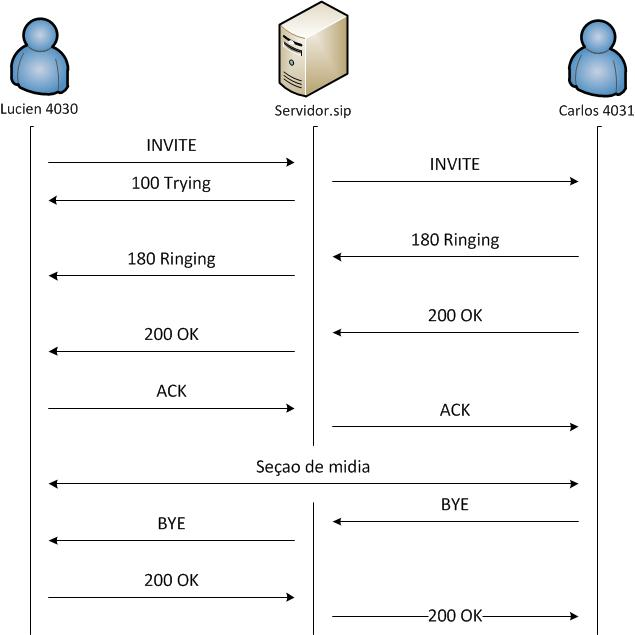
\includegraphics[width = 0.8\linewidth]{images/chamadaSIP}
  \caption{Exemplo de chamada SIP} %titulo da figura
  \label{f_mediaStream}
\end{figure}

\subsection{WebSockets}
\label{ss_webSockets}
A web tem sido construída com base no mecanismo de pedido e resposta de HTTP, ou seja, quando um usuário acessa uma página, nada irá acontecer até que ele clique em outra página para atualizar as informações desta. Mais tarde, o AJAX veio para deixar a web mais dinâmica. porém, toda a comunicação HTTP continuava sendo direcionada pelo cliente, o que ainda exigia interação do usuário ou  temporizador que atualizasse a página. 

A tecnologia que permite o servidor enviar dados atualizados para os clientes, e que foi utilizado por algum tempo, é conhecido como sondagem longa. Um dos principais problemas deste tipo de solução era o overhead de HTTP, que poderia prejudicar soluções que não são tolerantes a atrasos, como jogos on-line. Para solucionar este problema, surgiu então o WebSocket.

WebSocket é uma tecnologia que permite a comunicação full-duplex sobre um único soquete TCP, entre cliente e servidor web. Ou seja, há uma conexão persistente onde ambas as partes podem começar a enviar dados a qualquer momento

\begin{figure}[!htdb]
 \centering
  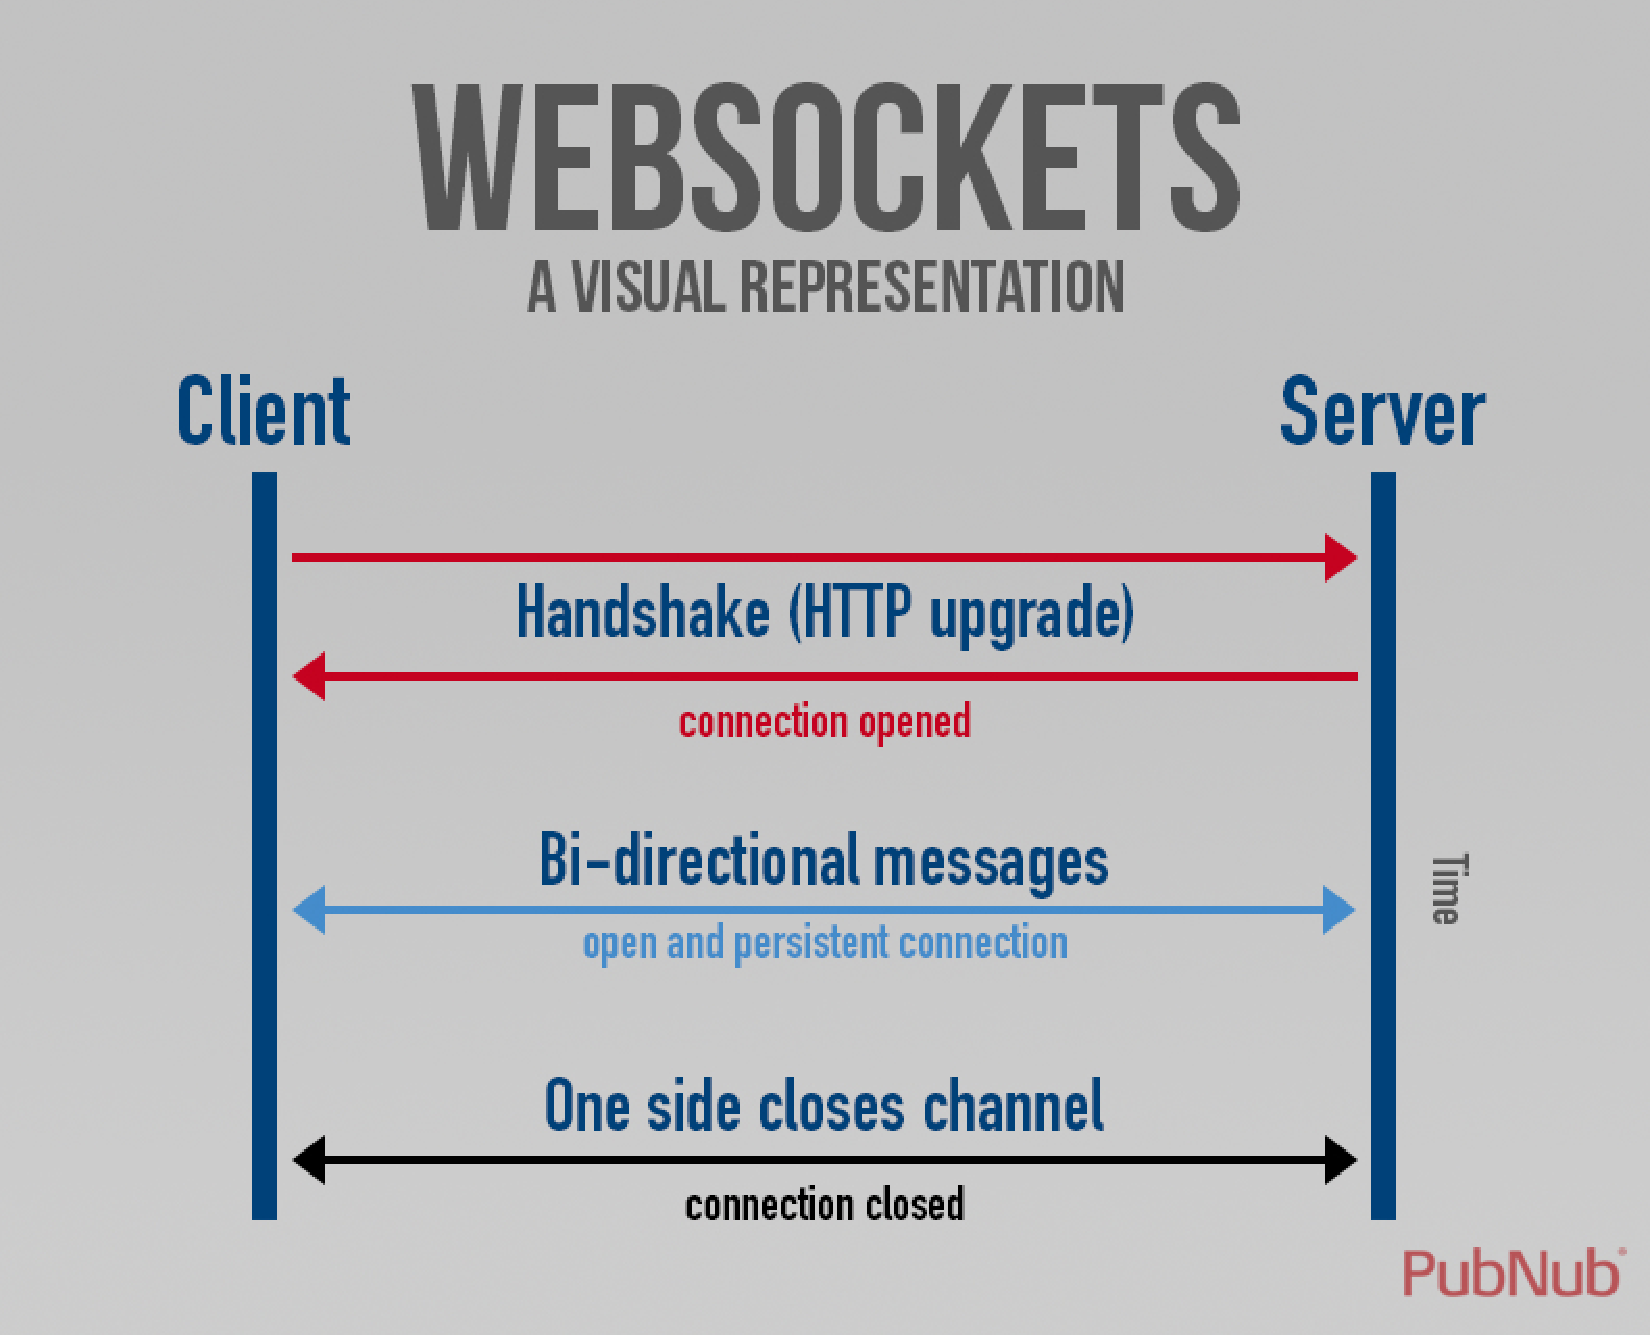
\includegraphics[width = 0.8\linewidth]{images/websocket}
  \caption{WebSockets} %titulo da figura
  \label{f_mediaStream}
\end{figure}

\subsection{SIP over WebSockets}
\label{ss_sipWebsockets}
SIP over Websockets é uma especificação que define um subprotocolo de Websocket, permitindo a troca de mensagens SIP entre um cliente e um servidor web. Assim como o SIP, ela é composta por algumas entidades \cite{Amaral:2013}. As duas principais são:

\begin{itemize}
  \item \textit{SIP WebSocket Client}: entidade responsável por abrir ligações de \textit{websockets} de saída para o servidor e que se comunica por \textit{WebSocket SIP subprotocol}.
  \item \textit{SIP WebSocket Server}: responsável por escutar ligações de entrada dos usuários e que se comunica por \textit{WebSocket SIP subprotocol}.
\end{itemize}


\section{Asterisk}
\label{s_asterisk}
O Asterisk é um software de código aberto, que implementa os recursos encontrados em um PABX convencional, utilizando a tecnologia VoIP. Foi desenvolvido e ainda é mantido pela empresa Digium (surgida em 1999). 
Atualmente, diversas empresas de pequeno a grande porte tem adotado este tipo de solução, pois permite o desenvolvimento de multiprotocolos a aplicações de comunicações em tempo real com voz e vídeo. Por ser código aberto, o software pode ser modelado de acordo com a necessidade da empresa.

Na versão 11 do Asterisk, foi adicionado o suporte ao WebRTC e criado o módulo res\underline{\hspace{.10in}}http\underline{\hspace{.10in}}websocket que permite programadores Javascript desenvolverem soluções em que haja interação e comunicação do WebRTC com o Asterisk. Dentro do módulo chan\underline{\hspace{.10in}}sip, foram adicionados WebSockets para permitir o uso de SIP como protocolo de sinalização. \cite{Amaral:2013}.

\section{Tecnologia auxiliares}
\label{s_tecAuxiliares}
Atualmente já existem algumas soluções WebRTC com funcionalidades diferentes que podem ser usadas e servir de base para outras aplicações. Uma delas é o SIPML5, que permitem a interoperabilidade entre soluções web e clientes SIP. 


\subsection{sipML5}
\label{ss_sipml5}

O sipML5 é uma aplicacao desenvolvida pela Doubango Telecom, que implementa a pilha do protocolo SIP em Javascript \cite{Borges:2013}. Pode ser usado em qualquer web browser, para uma ligação a uma rede SIP permitindo realizar e receber chamadas vídeo ou voz. Alguma das funções suportadas:

\begin{itemize} %Latex < List Environment
 \item chamadas vídeo e áudio;
 \item mensagens instantâneas;
 \item presença;
 \item transferência de chamadas;
 \item chamada em espera;
\end{itemize}

Seu uso, é recomendável no Google Chrome e Firefox stable. Nos demais navegadores, é necessário instalar a extensão \textit{webrtc4all}. Exemplo na figura 2.8.

\begin{figure}[!htdb]
 \centering
  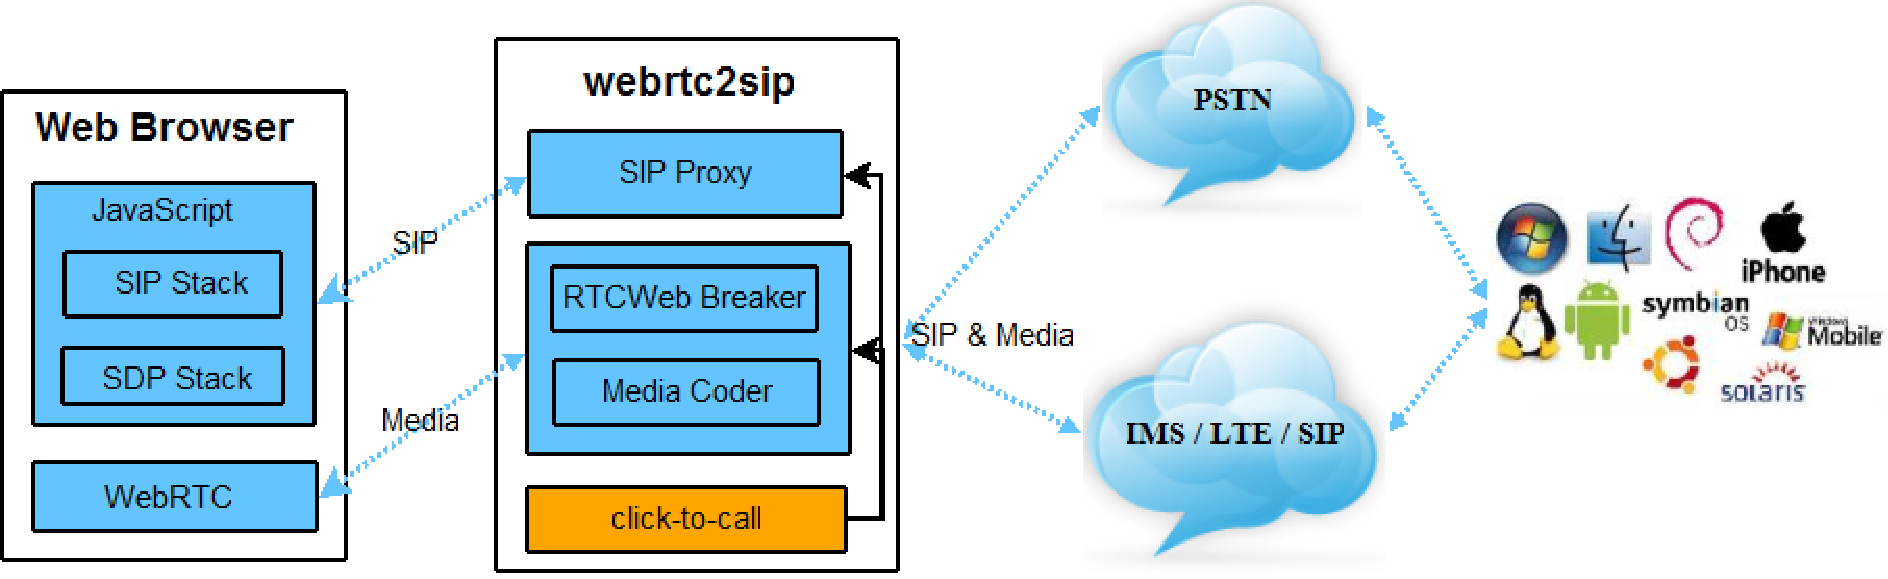
\includegraphics[width = 1\linewidth]{images/sipml5}
  \caption{Uso do sipML5} %titulo da figura
  \label{f_mediaStream}
\end{figure}

É importante ressaltar, que a partir da versão 11, o Asterisk tem suporte nativo ao WebRTC, dispensando o uso de um gateway como é o caso do \textit{WebRTC2SIP} que realiza a conversões dos pacotes enviados pelo endpoint que utiliza webRTC, no caso o SIPML5, para o PABX IP. Na figura 2.9 um pedaço do código responsável pela chamada entre dois usuários.


\begin{figure}[!htdb]
 \centering
  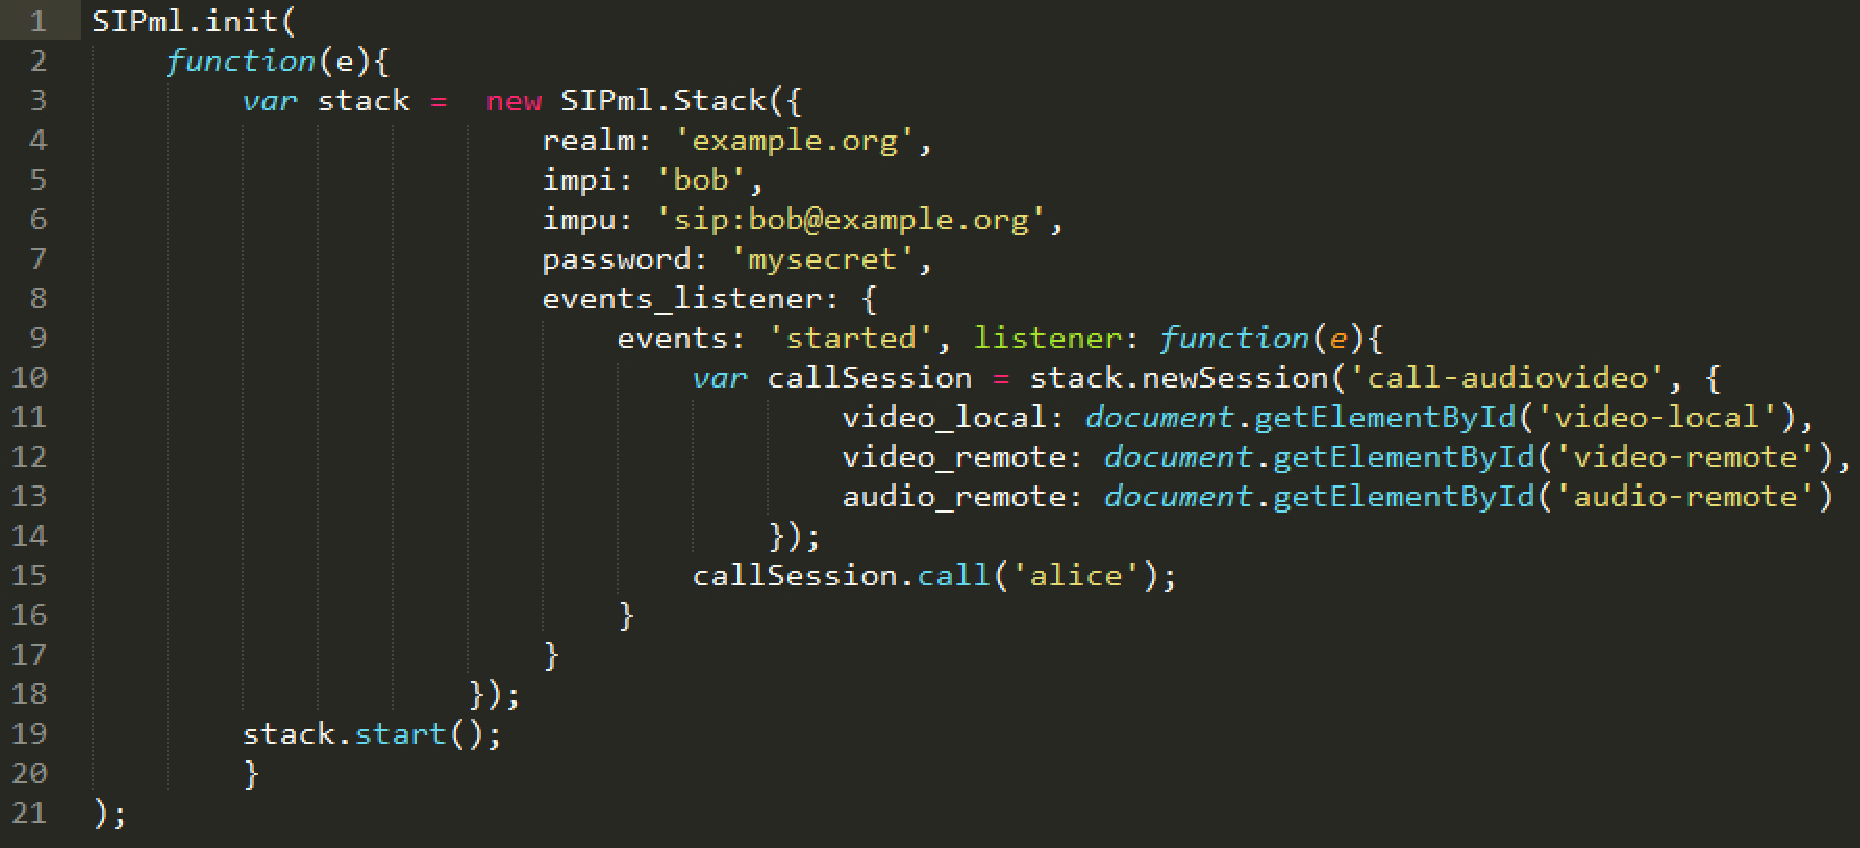
\includegraphics[width = 1\linewidth]{images/sipml5code}
  \caption{Inicialização da maquina, da pilha SIP e uma chamada de Bob para Alice no sipML5} %titulo da figura
  \label{f_mediaStream}
\end{figure}


\section{Linguagens utilizadas no projeto}
\label{s_linguagensProjeto}

\subsection{HTML5}
\label{ss_html5}
Criada por Tim Barners Lee na década de 1990, e com suas especificações controladas pela W3C \textit{World Wide Web Consortium}, o HTML \textit{HyperText Markup Language}, é uma linguagem  de marcação utilizada para produção de páginas na \textit{web}, que permite a criação de documentos que podem ser lidos em praticamente qualquer navegador.

Para escrever documentos HTML é necessário de apenas um editor de texto e conhecimento sobre a linguagem. Esta são compostas por tags servem para indicar a função de cada elemento da página \textit{web}. Os tags funcionam como comandos de formatação de textos, formulários, links, imagens, tabelas, entre outros.

O HTML versão 5, adiciona várias novas funções sintáticas, incluindo as tags de video e áudio que são indispensáveis para o funcionamento o WebRTC. Na figura 2.10 um simples exemplo utilizando as principais tags do HTML5.

\begin{figure}[!htdb]
 \centering
  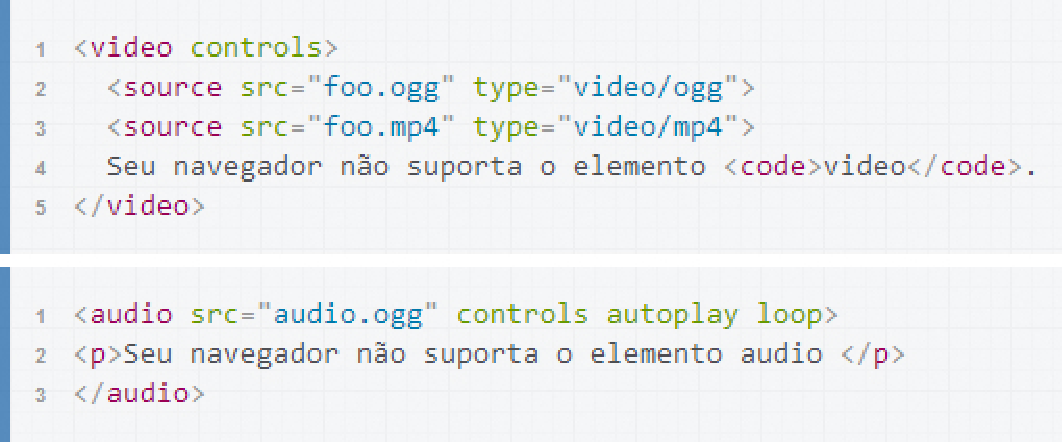
\includegraphics[width = 1\linewidth]{images/html5}
  \caption{Utilização de vídeo e áudio em uma página \textit{web}} %titulo da figura
  \label{f_mediaStream}
\end{figure}

\subsection{CSS}
\label{ss_css}
O CSS \textit{Cascading Style Sheets} é uma linguagem para estilos que define o layout de documentos HTML, ou seja, ela controla os tipos de  fontes, cores, alturas e larguras, posicionamento, entre outros elementos de uma página web. Foram criadas basicamente para deixá-las mais elegantes e atrativas aos usuários.

\subsection{Javascript}
\label{ss_javascript}
Criada por Brendan Eich e lançado pela primeira vez na versão beta do navegador NetScape 2.0 em 1995, o Javascript é uma linguagem programação interpretada no lado cliente, ou seja, é processada pelo próprio navegador. Com o JavaScript podemos criar efeitos especiais para nossas páginas na Web, além de proporcionar uma maior interatividade com nossos usuários. \cite{JAVASCRIPT}
Hoje o Javascript é considerado a principal linguagem para programação client-side em navegadores web e todos os exemplos de códigos aqui apresentados, o utilizam. 

\chapter{Proposta} % artigo é dividido por sessões
\label{c_bibliografia} % serve para referência cruzada

A proposta deste trabalho é implementar uma aplicação onde um usuário que esteja utilizando um simples navegador \textit{web}, consiga realizar chamadas para pontos finais que estejam utilizando SIP, como por exempo ATA's, telefones IP, \textit{softphones}, entre outros. Deverá também mostrar quais usuários que estão disponíveis no momento, ocupados ou desconectados.
Para isso, dever ser feita uma integração da aplicação desenvolvida juntamente com o servidor Asterisk.

Ao final do projeto, será realizado alguns testes de desempenho para avaliar a qualidade das ligações.

\section{Cenário}
\label{s_cenario} %serve para referência cruzada

O cenário pensado para a implementação da aplicação e realização de testes, está logo abaixo na figura 3.1. A versão do Asterisk que será utilizado é a versão 11 ou superior, pois nativamente já possui suporte para o WebRTC. Na parte do \textit{WebServer} rodando a aplicação, será utilizado como base o sipML5, pois este já implementa a pilha do protocolo SIP em Javascript, disponibilizando ligações a uma rede SIP. Toda a questão de sinalização, também é mostrada na figura.

\begin{figure}[!htdb]
 \centering
  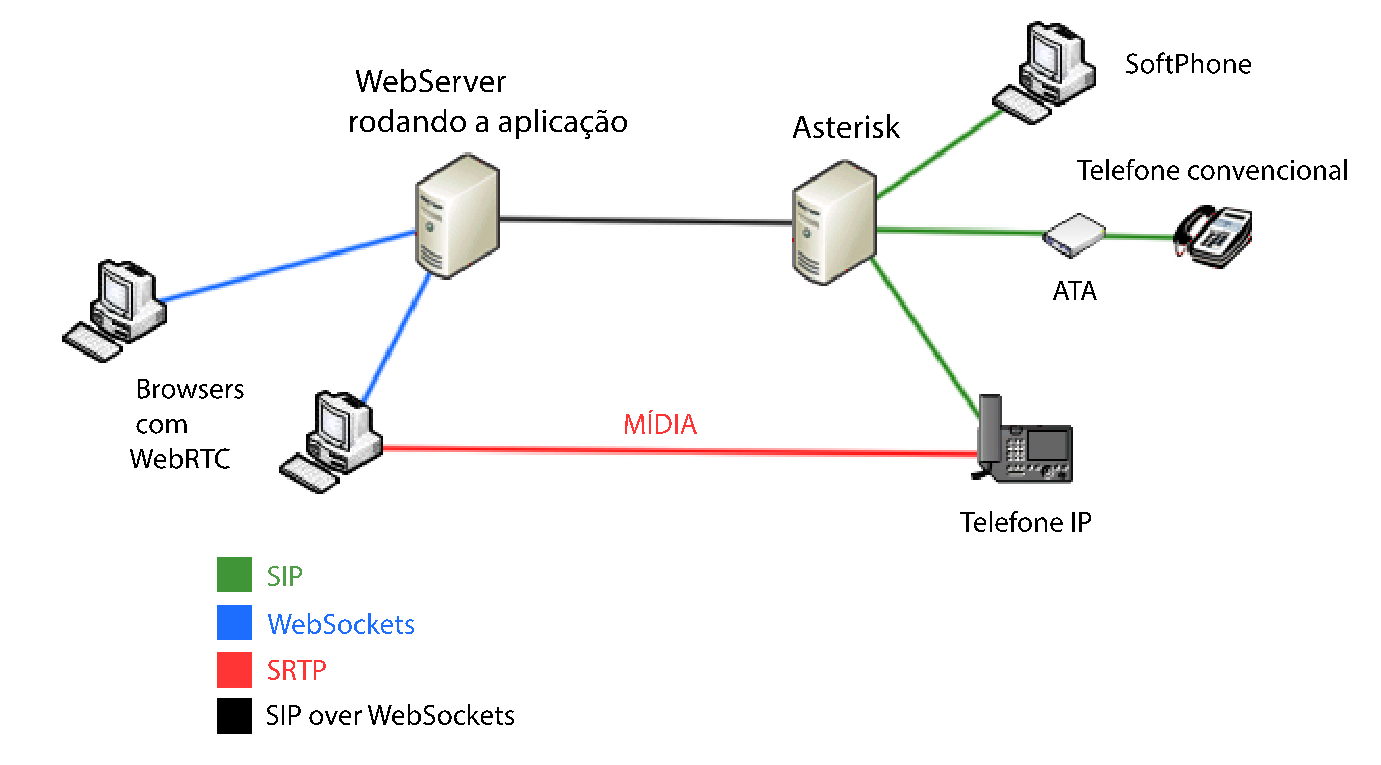
\includegraphics[width = 1\linewidth]{images/cenario}
  \caption{Cenário básico para realização de testes} %titulo da figura
  \label{f_cenario}
\end{figure}

\section{Ambiente de experimentação}
\label{s_ambienteDeExperimentacao} %serve para referência cruzada

Para realização de testes, será utilizado máquinas virtuais que farão papel de cliente e servidor, simulando cenários próximo do real. Posteriormente será realizado testes na rede do campus IFSC-SJ.

\section{Ambiente de desenvolvimento}
\label{s_ambienteDeDesenvolvimento} %serve para referência cruzada

Como a Web API do WebRTC foi implementada em Javascript, para criar soluções a partir dela, será necessário apenas de um editor de texto, que neste caso será o Sublime Text 2. Ferramenta gratuita com grande poder de customização.

\section{Cronograma}
\label{s_cronograma} %serve para referência cruzada

\begin{table}[!htpb]
\centering

% definindo o tamanho da fonte para small
% outros possíveis tamanhos: footnotesize, scriptsize
\begin{small} 
  
% redefinindo o espaçamento das colunas
\setlength{\tabcolsep}{3pt} 

% \cline é semelhante ao \hline, porém é possível indicar as colunas que terão essa a linha horizontal
% \multicolumn{10}{c|}{Meses} indica que dez colunas serão mescladas e a palavra Meses estará centralizada dentro delas.

\begin{tabular}{|c|c|c|c|c|c|c|c|c|c|c|c|c|c|c|c|c|c|c|c|c|c|c|c|c|}\hline
 & \multicolumn{12}{c|}{Meses}\\ \cline{1-13}
\raisebox{1.5ex}{Etapa} & 01 & 02 & 03 & 04 & 05 & 06 & 07 & 08 & 09 & 10 & 11 & 12 \\ \hline

Pesquisa Bibliográfica &  &  & X & X & X &  &  &  &  &  &  & \\ \hline
Escrita de relatório de TCC1 &  &  &  &  &  & X &  &  &  &  &  & \\ \hline
Entrega do Documento e Apresentação TCC1 &  &  &  &  &  &  & X &  &  &  &  & \\ \hline
Desenvolvimento do projeto &  &  &  &  &  &  & X & X & X & X & X & X \\ \hline
Elaboração do Documento de Avaliação Final &  &  &  &  &  &  & X & X & X & X & X & X  \\ \hline

\end{tabular} 
\end{small}
\caption{Cronograma das atividades previstas}
\label{t_cronograma}
\end{table}

%\chapter{Considerações finais} % artigo é dividido por sessões
%\label{c_consideracoesFinais} % serve para referência cruzada

\nocite{*}

\bibliographystyle{abnt}
\bibliography{ref}

\end{document}

